
\chapter{System architecture of HyCube - a distributed hash table based on a variable metric}
\label{sec:hycubeArchitecture}

This chapter presents the routing architecture of \emph{HyCube} - a distributed hash table system based on a hierarchical hypercube geometry. Sections \ref{sec:hycubeHierarchicalHypercube} and \ref{sec:hycubeRoutingTables} introduce the hierarchical hypercube concept and describe the structure of routing tables maintained by nodes. Section \ref{sec:routing} presents the basic routing algorithm, and the subsequent sections present various optimizations of the routing algorithm. The optimizations of the basic routing algorithm include the use of a variable routing metric (defining distances between nodes) adopting Steinhaus transform (Section \ref{sec:metric}) - the routing metric is modified by nodes on routes in a way resulting in a very high degree of flexibility in next hop selection (and this a very high level of resilience to node failures), preserving the routing efficiency of the basic algorithm. The concepts presented in this document have been published in \cite{hycubePpam2009} and \cite{hycubeICSReportFeb2013}.





\section{Hierarchical hypercube geometry}
\label{sec:hycubeHierarchicalHypercube}

The routing geometry of \emph{HyCube} is a combination of the tree geometry and the hypercube geometry. It is similar to \emph{Plaxton mesh} \cite{plaxton1}, \cite{plaxton2}, but nodes are also logically located in vertices of a $d$-dimensional hierarchical hypercube. A hierarchical hypercube is a hypercube whose vertices are also (lower level) hypercubes. Vertices of the hypercubes at the lowest level are positions which may be assigned to nodes. 

\begin{figure}
\centering
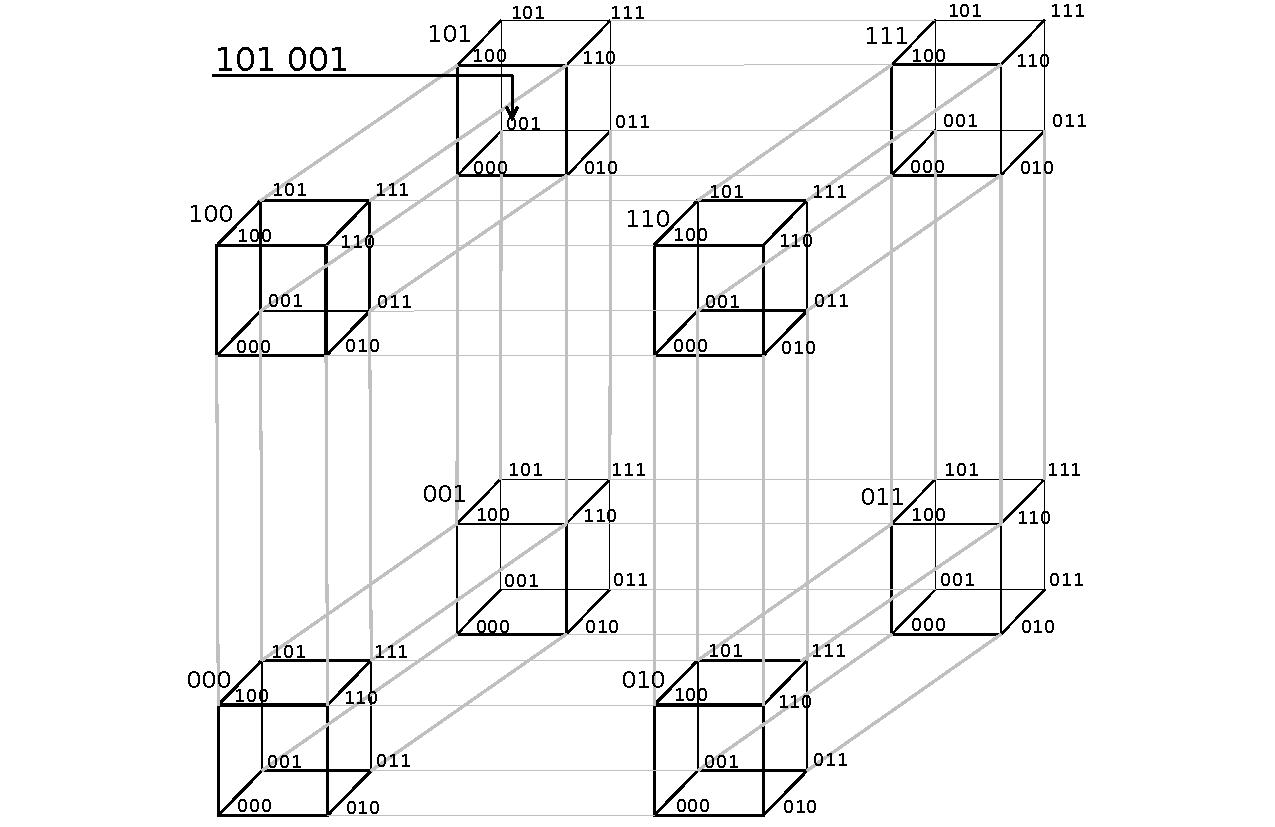
\includegraphics[scale=.6]{img/hh.pdf}
\caption{A hierarchical hypercube (3 dimensions and 2 levels of hierarchy)}
\label{fig:hierarchicalHypercube}
\end{figure}

Figure \ref{fig:hierarchicalHypercube} presents the structure of an exemplary hierarchical hypercube with 3 dimensions and 2 hierarchy levels. Node IDs are determined by their positions - the identifier of a node is a string of $d$-bit groups determining positions of the node in hypercubes at individual levels (starting with the hypercube at the highest level). The position in a hypercube at a particular level is a number built of bits corresponding to the positions of the node in the hypercube in individual dimensions. The length of the identifier equals $d \cdot l$, where $d$ is the number of dimensions, and $l$ is the number of levels.

The hierarchical hypercube and the tree geometries are isomorphic. However, visualizing the structure as a hierarchical hypercube gives an idea of the spatial arrangement of nodes in a $d$-dimensional space - the numbers formed from bits corresponding to individual dimensions relate to the coordinates of the node in these dimensions in the system of coordinates with the center in point $0$. Thus, considering the ID space as a segment of $\mathbb{Z}^d$ space ($\mathbb{Z}$ denotes the set of integer numbers), the distance between nodes may be defined by any metric applicable to $\mathbb{Z}^d$, or $\mathbb{R}^d$ ($\mathbb{R}$ - the set of real numbers) as $\mathbb{Z}$ is a subset of $\mathbb{R}$. However, the geometry of \emph{HyCube} should be seen as a $d$-dimensional torus with the perimeter equal to $2^l$ in each dimension (the set of coordinates in each dimension is treated as on a ring). That means that after the point $2^l-1$, point $0$ is located, and all arithmetic is done modulo $2^l$. This fact is important in determining distances between nodes - in every dimension the distance is determined like on a ring - it is the shorter of the distances in either direction.

In \emph{HyCube}, the default number of dimensions is 4 and the number of levels is 32, resulting in a 128-bit address space (which allows avoiding conflicts of identifiers in majority of applications).



\section{Routing tables}
\label{sec:hycubeRoutingTables}

\subsubsection{Primary routing table.}

The primary routing table has the same structure as in \emph{Plaxton mesh}. It has $l$ levels (the number of hierarchy levels), and, at each level, there are $2^d$ slots ($d$ - the number of dimensions). In the primary routing table of a node $X$, the slot $j$ at level $i$ ($i \geq 0$) contains a reference to a node that is located in the same hypercube at level $i+1$ and in the hypercube corresponding to the number $j$ at level $i$ (lower level). At each level $i>0$, one slot corresponds to the hypercube in which the node $X$ is located - this slot is left empty, as the routing table contains a whole level corresponding to this hypercube.

An exemplary primary routing table for a 2-dimensional hierarchical hypercube with 6 hierarchy levels for node $X$ = 112013 is presented in Table \ref{tab:rt1Example}. For clarity, groups of bits are represented by quaternary digits (base-4 numeral system). The digits in bold represent the sub-hypercube addresses corresponding to routing table slots at individual levels. The underlined digits represent the hypercubes corresponding to the routing table slots matching the hypercubes of node $X$ at individual levels.

\begin{table}
\scriptsize
\begin{center}
%\begin{tabular}{p{2cm}|p{1.3cm}|p{1.3cm}|p{1.3cm}|p{1.3cm}|}
\begin{tabular}{c|c|c|c|c|}
	\hhline{*{1}{~}*{4}{|-}|~|}
																				& \texttt{\textbf{0}}									& \texttt{\textbf{1}}											& \texttt{\textbf{2}}											& \texttt{\textbf{3}}										\\
    \hline
    \multicolumn{1}{|c|}{\texttt{\textbf{Level 5}}}								& \texttt{\underline{\textbf{0}}11033}					& \texttt{-}													& \texttt{\underline{\textbf{2}}31011}							& \texttt{\underline{\textbf{3}}00232}						\\
	\multicolumn{1}{|c|}{\texttt{\textbf{Level 4}}}								& \texttt{\underline{1\textbf{0}}2223}					& \texttt{-}													& \texttt{\underline{1\textbf{2}}1301}							& \texttt{\underline{1\textbf{3}}0001}						\\
	\multicolumn{1}{|c|}{\texttt{\textbf{Level 3}}}								& \texttt{\underline{11\textbf{0}}113}					& \texttt{\underline{11\textbf{1}}201}							& \texttt{-}													& \texttt{\underline{11\textbf{3}}302}						\\
	\multicolumn{1}{|c|}{\texttt{\textbf{Level 2}}}								& \texttt{-}											& \texttt{\underline{112\textbf{1}}01}							& \texttt{\underline{112\textbf{2}}03}							& \texttt{\underline{112\textbf{3}}12}						\\
	\multicolumn{1}{|c|}{\texttt{\textbf{Level 1}}}								& \texttt{\underline{1120\textbf{0}}3}					& \texttt{-}													& \texttt{\underline{1120\textbf{2}}1}							& 															\\
	\multicolumn{1}{|c|}{\texttt{\textbf{Level 0}}}								& 														& 																& 																& \texttt{-}												\\
    \hline
\end{tabular}
\end{center}
\caption{Exemplary primary routing table for node 112013 (for a 2-dimensional hierarchical hypercube with 6 hierarchy levels).}
\label{tab:rt1Example}
\end{table}




\subsubsection{Secondary routing table.}

The secondary routing table of a node $X$ contains nodes from adjacent hypercubes to the hypercube of node $X$ in each dimension, in both directions, at each level. An adjacent hypercube (at any level) is the one whose coordinate in one dimension is greater or smaller by 1 than the coordinate of the same level hypercube of $X$ (modulo $2^l$), and coordinates in all other dimensions are equal to those of $X$. The secondary routing table does not contain nodes in slots at the highest level, as hypercubes corresponding to them are covered by the primary routing table. Also, one of the adjacent hypercubes at each level in each dimension is covered by a primary routing table slot.

The secondary routing table increases the level of flexibility in the next hop selection. If the distance between nodes is defined by a metric in $\mathbb{R}^d$ space, it is very likely that the secondary routing table contains nodes that are closer to any arbitrarily chosen node. Furthermore, it provides additional shortcut references when a message is routed to a node that is close in the $\mathbb{R}^d$ space, but is not close in terms of the \emph{Plaxton mesh} distance. With the use of the primary routing table, routing a message between nodes sharing a short ID prefix would require many steps of traversing the tree structure.

Table \ref{tab:rt2Example} presents an exemplary secondary routing table for node $X$ = 113012 (binary 01'01'11'00'01'10) - for a 2-dimensional hierarchical hypercube with 6 hierarchy levels. For clarity, in this example, the IDs are represented as binary numbers. Addresses of adjacent hypercubes corresponding to the routing table slots are marked in bold, and bits of addresses of adjacent hypercubes corresponding to the particular dimension are underlined - the numbers built of these bits are larger by 1 or smaller by 1 than the numbers formed of the corresponding bits of $X$. All other hypercube address bits (the remaining dimensions) are equal to the corresponding ones of $X$.

\begin{table}
\scriptsize
\begin{center}
%\begin{tabular}{p{1.7cm} p{2.7cm} p{2.7cm} p{2.7cm} p{2.7cm}}
\begin{tabular}{c|c|c|c|c|}
    \hhline{*{1}{~}*{4}{|-}|~|}
														& \multicolumn{2}{c|}{\texttt{\textbf{Dimension 0}}}																																		& \multicolumn{2}{c|}{\texttt{\textbf{Dimension 1}}} 																																							\\
    \hhline{*{1}{~}*{4}{|-}|~|}
														& $\leftarrow$																			& $\rightarrow$																						& $\leftarrow$																						& $\rightarrow$																						\\
	\hline
    \multicolumn{1}{|c|}{\texttt{\textbf{Level 5}}}		& \texttt{-}																			& \texttt{-}																						& \texttt{-}																						& \texttt{-}																						\\
	\multicolumn{1}{|c|}{\texttt{\textbf{Level 4}}}		& \texttt{\textbf{0\underline{1}'0\underline{0}}'01'01'00'11}							& \texttt{\textbf{0\underline{0}'0\underline{0}}'10'01'10'10}										& \texttt{\textbf{\underline{1}1'\underline{1}1}'10'01'00'11}										& \texttt{\textbf{\underline{0}1'\underline{1}1}'00'10'10'01}										\\
	\multicolumn{1}{|c|}{\texttt{\textbf{Level 3}}}		& \texttt{\textbf{0\underline{1}'0\underline{1}'1\underline{0}}'10'01'00}				& \texttt{\textbf{0\underline{0}'0\underline{0}'1\underline{0}}'11'01'01}							& \texttt{\textbf{\underline{0}1'\underline{0}1'\underline{0}1}'11'01'01}							& \texttt{\textbf{\underline{0}1'\underline{1}1'\underline{0}1}'01'00'01}							\\
	\multicolumn{1}{|c|}{\texttt{\textbf{Level 2}}}		& \texttt{\textbf{0\underline{1}'0\underline{1}'1\underline{0}'0\underline{1}}'11'10}	& \texttt{\textbf{0\underline{1}'0\underline{1}'1\underline{1}'0\underline{1}}'01'01}				& \texttt{\textbf{\underline{0}1'\underline{0}1'\underline{0}1'\underline{1}0}'01'10}				& \texttt{\textbf{\underline{0}1'\underline{0}1'\underline{1}1'\underline{1}0}'10'00}				\\
	\multicolumn{1}{|c|}{\texttt{\textbf{Level 1}}}		& 																						& \texttt{\textbf{0\underline{1}'0\underline{1}'1\underline{1}'0\underline{1}'0\underline{0}}'10}	& \texttt{\textbf{\underline{0}1'\underline{0}1'\underline{0}1'\underline{1}0'\underline{1}1}'00}	& \texttt{\textbf{\underline{0}1'\underline{0}1'\underline{1}1'\underline{0}0'\underline{1}1}'10}	\\
	\multicolumn{1}{|c|}{\texttt{\textbf{Level 0}}}		& 																						& 																									& 																									& 																									\\
     \hline
\end{tabular}
\end{center}
\caption{Exemplary secondary routing table for node 113012 (01'01'11'00'01'10) - for a 2-dimensional hierarchical hypercube with 6 hierarchy levels.}
\label{tab:rt2Example}
\end{table}



\subsubsection{Neighborhood set (closest neighbors set).}


In addition to the routing tables described above, nodes maintain sets of closest to them (according to the chosen metric) nodes existing in the system - called \emph{neighborhood sets}. These sets may allow finding a next hop (routing/lookup), decreasing the distance left to the destination, even if there are no appropriate nodes in both routing tables. The closest neighbors sets are expected to increase the probability of delivering messages in the presence of node failures. The neighborhood sets have also very good properties for supporting joining and leaving procedures, as well as maintenance and recovery algorithms, and they help to keep the DHT consistent. Moreover, their existence is crucial for searching closest nodes for a given key, as well as for replicating resources, which will be discussed in detail in Chapters \ref{sec:lookupSearch} and \ref{sec:resourcesManagement}. In \emph{HyCube}, the default size of the neighborhood set is 16.








\section{Basic routing algorithm}
\label{sec:routing}

Let us consider routing a message from node $X$ to node $Y$. Every node $R$ along the route first checks if there is a reference to the destination node in its neighborhood set, in which case, the message is sent directly to that node. Otherwise, the routing tables are searched for an appropriate next hop - the node that shares at least one $d$-bit group longer prefix of ID with $Y$ (than with $R$) or shares the same number of $d$-bit groups of the ID but is closer to $Y$ than $R$ in terms of the chosen routing metric. The routing metric of \emph{HyCube} is discussed in Section \ref{sec:metric}. For the time being, let us assume that routing converges according to the Euclidean metric. The detailed algorithm is presented below:

\begin{enumerate}

\item Initially, the routing algorithm finds the slot in the primary routing table that corresponds to nodes sharing at least one group of $d$ bits longer prefix of ID with $Y$ than with the current node ($R$). In a hierarchical hypercube, this slot corresponds to a hypercube in which the destination node is located, at a lower level than the lowest-level hypercube containing both, the current and the destination node. If for the current node and $Y$, the common prefix length equals $i$, and the next $d$-bit group of the ID of $Y$ equals $j$, $j$-th routing table slot at level $l - 1 - i$ is used. If this slot is not empty, the message is routed to the node found in the slot - increasing the common prefix length with the destination node $Y$ by at least one $d$-bit group.

\item If no node is found in the appropriate primary routing table slot, nodes sharing the same prefix length with $Y$ as with $R$ (in terms of the number of bit groups), but closer to $Y$ in terms of the chosen metric, are also considered - both routing tables and the neighborhood set are checked. From the set of nodes found, the node sharing the longest prefix of the ID with $Y$ (number of $d$-bit groups) is chosen, and, if there are more than one such nodes, the node closest to $Y$ (according to the routing metric) is chosen for the next hop.

\end{enumerate}

The primary routing table supports routing based on extending the ID prefix (in terms of $d$-bit groups) - tree-based routing (\emph{Plaxton mesh}), and the secondary routing table supports finding a closer node in any dimension - such nodes are likely to be closer to the destination node also in terms of the Euclidean metric. Both routing tables and the neighborhood set are used for determining the best possible next hop, to which the message is routed.

It can be shown that the expected route length equals $\lceil\log_{2^d} N\rceil$ hops and, on average, $\lceil\log_{2^d} N\rceil \cdot (2^d-1)$ slots are populated in the primary routing table and $(\lceil\log_{2^d} N\rceil - 1) \cdot d$ in the secondary routing table ($N$ is the number of nodes in the network)\footnote{Based on the assumption that nodes are uniformly distributed in the hierarchical hypercube}.




\subsubsection{Message TTL}

To limit the maximum number of hops for messages, every message contains the TTL information (determining the maximum number of hops) and the number of hops that the message already passed. The TTL value should be decremented, and the number of hops is incremented by every node along the route (including the initiating node) before passing it to the next hop. When the TTL falls below 0, after decrementing, the message should not be routed any further and be dropped.



\subsubsection{Acknowledging message delivery and detecting duplicates}

Optionally, after receiving messages (DATA messages - sent at the application level), depending on configuration, nodes may send acknowledgments (DATA\_ACK messages) confirming receiving of the messages (either directly to the sending node, or routed via the system to the message sender). When the sending node receives the DATA\_ACK message, it knows that the original message was successfully received and processed, and, when no acknowledgment is received (timeout), the node might resend the message (automatic resending may also be configured - up to the defined maximum number of retries). In cases when the acknowledgment mechanism is implemented at the application level (beyond the scope of \emph{HyCube}), the native \emph{HyCube} mechanism may be switched off.

\emph{HyCube} also implements message duplicate detection. In case of receiving a message duplicate, the duplicate is dropped. Message duplicates may be received as a result of incorrect routing or network problems, or an ACK message not being delivered. Duplicates are detected based on the header of the message (the details are specified in Chapter \ref{sec:protocol}).






\section{Number of dimensions versus number of levels}

The address (node identifiers) space should be large enough to prevent potential conflicts of identifiers (existence of two nodes with the same ID). The size of the address space in \emph{HyCube} equals:

\begin{equation}
N_{max} = 2^{d \cdot l}
\end{equation}

\noindent
which means that increasing the number of dimensions or the number of hierarchy levels would increase the number of possible identifiers that nodes may be assigned. However, the number or dimensions and levels of the hierarchical hypercube influences the system characteristics.

Adding additional levels of hierarchy causes the address space to increase, but it also proportionally increases the number of routing table slots that nodes maintain. Moreover, the pessimistic route length would also increase, as in the pessimistic scenario, routing steps correspond to individual routing table levels. Nevertheless, the expected route length remains at the same level, because, on average, similar number of routing table slots would be populated (with high probability the lower-level slots are empty).

Increasing the number of dimensions, on the other hand, has a very strong impact on routing characteristics. Although the routing tables grow sharply with the increase of the number of dimensions, the routing algorithm is more specific in selecting next hops - in each routing step, the common prefix with the destination node ID is increased by a larger number of bits, maintaining the same pessimistic path length and decreasing the average path length. As the base of the logarithm (Equation \ref{equ:expPathLenRT1}) grows exponentially, the expected path length is inversely proportional to the number of dimensions:

\begin{equation}
\label{equ:expPathLenRT1}
\log_{2^d} N = \frac{1}{d} \log_2 N
\end{equation}

\noindent
However, the maintenance cost is significant, as the primary routing table size grows exponentially with the number of dimensions:

\begin{equation}
\log_{2^d} N \cdot (2^d-1) = \frac{\log_{2} N \cdot (2^d-1)}{d}
\end{equation}

At one extreme, when the number of dimensions is equal to the number of identifier bits (1 level of hierarchy), every node would maintain references to all other nodes in the system, and the routing table slots would correspond to all possible values of node identifiers. Increasing the number of dimensions may influence any algorithm used in the distributed hash table and may require adjusting the parameter values for the specified number of dimensions. That is why it is crucial to determine a reasonable value for the number of dimensions that would ensure good routing properties and reasonable sizes of the routing tables, while controlling the identifier length should be done by increasing/decreasing the number of hierarchy levels. Whenever the number of dimensions is changed, it should be verified again that the DHT algorithms parameters still have their optimal values.










\section{Routing table nodes selection}
\label{sec:HyCubeNodeSelection}

The routing table node selection technique used in \emph{HyCube} is a variant of the LNS approach, which, at the same time, provides means to remove failed nodes from routing tables.


\subsubsection{LNS (liveness node selection) in HyCube}
\label{sec:HyCubeNodeSelectionLNS}

\emph{HyCube} uses a variant of LNS which bases the neighbor choice on node liveness information discovered locally, working together with a background process checking node's responsiveness. However, the \emph{HyCube} LNS implementation does not calculate the liveness information based on the node's join and leave times. Every node periodically sends keepalive (PING) messages to all the nodes in its routing tables and updates the stored nodes' liveness values. The value is increased when the node responds to the PING message (sending a PONG message), and is decreased if the keepalive response is not received (timeout). The initial liveness value (new nodes) is defined by the system parameter $L_{init}$, and the values are updated as follows:

\begin{equation}
L = L_{prev} \cdot p + (1-p) \cdot L_{max}
\end{equation}

\noindent
if the keepalive confirmation (PONG message) was received, or:

\begin{equation}
L = L_{prev} \cdot p
\end{equation}

\noindent
when the keepalive fails (no PONG message is returned). $L_{prev}$ is the previous value of liveness, $L$ is the new, updated liveness value, $L_{max}$ and $p$ are system parameters. When $L$ falls below the threshold value $L_{deactivate}$ (system parameter), the node is marked as deactivated and is not used in the routing procedure until $L$ falls below the threshold value $L_{remove}$ (parameter), in which case the node is permanently removed from routing tables, or until $L$ reaches above $L_{deactivate}$ again. Whenever the value of $L$ is below the value of the parameter $L_{replace}$, when possible, the current node in the routing table slot is replaced by a new node, whose value $L$ is then given the initial value $L_{init}$. The value of $L$ for any node removed from the routing table should however be stored by nodes for some time to prevent replacing new nodes that temporarily fall below $L_{replace}$ with nodes that were permanently unresponsive. The values $0 < p < 1$ (update coefficient), $L_{deactivate}$, $L_{replace}$ and $L_{remove}$ determine the sensitivity of the algorithm, and $L_{max}$ defines the maximum value of $L$. This technique provides a good way to keep long-living responsive nodes in routing tables and eliminate failed or overloaded nodes that are not able to handle requests. Reasonable values of $p$, $L_{deactivate}$, $L_{replace}$ and $L_{remove}$ should be chosen to prevent the algorithm from removing nodes from routing tables in case of temporary delays in sending responses by nodes, but still, to be able to efficiently remove failed nodes. If $L_{max} = 2$, the values of $L_{init} = 1.5$, $p = 0.5$, $L_{deactivate} = 1$, $L_{replace} = 0.5$ and $L_{remove} = 0.05$ are good defaults as they allow avoiding failed paths due to temporary nodes' unresponsiveness, at the same time allowing unresponsive nodes to be replaced by new nodes. Using these default values would cause deactivating nodes after a single failed keep-alive, however, not replacing/removing them immediately. The parameter values (as well as the keep alive interval) may be fine-tuned depending on the system characteristics. The flexibility in next hop selection guaranteed by \emph{HyCube} ensures that no significant increase in failed paths rate, nor the average path length, is observed even if large portions of nodes temporarily do not respond to keep-alive messages and are deactivated.




\subsubsection{\emph{HyCube} mixed mode node selection}

The LNS technique described above allows replacing a routing table node only when its value of $L$ drops below $L_{replace}$ (or when $L$ reaches $L_{remove}$, in which case the node is removed). In some cases, however, it would be desirable to take another criterion (or criteria) into account, like for example proximity or any application specific measure. To achieve that, the condition $L < L_{replace}$ may be relaxed, and the neighbor selection could be based on a function measuring both factors - the liveness and the second factor (algorithm-specific). The liveness fulfillment factor may be defined as follows:

\begin{equation}
	Fact_{L} = \left|\frac{L - L_{replace}}{L_{replace}}\right|^{e_L} \cdot \mathop{\mathrm{sgn}}(L - L_{replace})
\end{equation}

\noindent
where the exponent $e_L$ determines the exponential growth of $Fact_{L}$ depending on the difference $L - L_{replace}$. Depending on the algorithm, this factor may be used to calculate overall criteria fulfillment at a node level, improvement of the criteria fulfillment for a new node, relative to current node(s), or may be used in calculating the quality function value for a set of nodes (for example for the neighborhood set). An exemplary neighbor selection criterion at a node level might be a weighted sum of two factors:

\begin{equation}
	Q = \alpha \cdot Fact_{L} + \beta \cdot Fact_{X}
\end{equation}

\noindent
where $Fact_{X}$ may be any neighbor selection algorithm specific function.







\section{Prefix mismatch heuristic}
\label{sec:pmh}

In the final part of a route, when the message is already relatively close to the destination node, the routing algorithm may omit some nodes that are close to the destination, but do not share the same long or longer prefix of ID with the destination node than with the current node. This phenomenon becomes more significant when a multidimensional metric is used. That is why, like in \cite{pastry}, \emph{HyCube} uses a heuristic switching to routing based only on the distance left, when a message is already in vicinity of the destination. Nodes should therefore be able to determine how close the message is to the destination in relation to the density of nodes in the space. In \emph{HyCube}, before choosing the next hop, each node checks if the distance to the destination is shorter than the average distance to the nodes in the neighborhood set multiplied by the factor $\lambda$: 

\begin{equation}
d_{dest} < \mathop{\mathrm{avg}}(d_{neigh}) \cdot \lambda
\end{equation}

\noindent
If this condition is satisfied, all further nodes on the route are chosen based only on their distance to the destination node - they might not share the same long or longer prefix of the identifier. All nodes from both routing tables and the neighborhood set are checked and the closest node is chosen for the next hop.

The prefix mismatch heuristic may be also enabled, when no next hop is found with routing based on extending the common prefix length with the destination node. This behavior may be configured by changing a system parameter value. In many cases, the number of neighborhood set nodes matching the destination is much larger if the selection is based only on the distance. Obeying the prefix condition is a much stronger constraint on the next hops, and may cause more failed paths, especially in the presence of many node failures. Thus, although the path length might increase, by default, \emph{HyCube} switches to routing based only on the distance left whenever no next hop is found. To maintain routing convergence, the prefix mismatch heuristic is followed by all subsequent nodes along the path.

The greater is the value of $\lambda$, the longer parts of routes will be determined based only on the distance left. The value should be large enough to ensure high probability of message delivery. However, too large values of $\lambda$ could cause an increase in path lengths. The performed simulations indicated that the value $\lambda = 1.5$ ensures good static resilience, maintaining the path lengths at a low level.





\section{Routing metric}
\label{sec:metric}

In DHT systems, distances between pairs of nodes are defined by a certain metric, and the routing converges according to this metric. The choice of the metric has a great impact on the average route length and the probability of message delivery. \emph{HyCube} uses a variable multi-dimensional metric adopting the Steinhaus transform, described in this section. It was confirmed during simulations that such an approach allows reaching a very high level of resilience to node failures and short pessimistic and average routing/lookup paths.




\subsection{Steinhaus transform}
\label{sec:steinhaus}

In \cite{nearNeighSearchMetrSpDim} and \cite{geomCutsMetrics}, the authors present the Steinhaus transform. The terminology comes from the fact that this distance was used in biological problems for the study of biotopes \cite{certDistSetsCorrDistOfFunc}. The theorem presented says that if $D$ is a metric on a set $X$, $D'$ is also a metric on $X$ for any $a \in X$, where:

\begin{equation}
\label{equ:steinhaus}
D'(x,y) = \frac{2D(x,y)}{D(x,a) + D(y,a) + D(x,y)}
\end{equation}

The default base metric used in \emph{HyCube} ($D$ in the equation above) is the Euclidean metric. Applying a metric with the Steinhaus transform to every route, setting the value of $a$ to the ID of the source node, causes the next hops to be chosen in such a way that they are closer to the destination node and more distant from the source node. Such an approach increases the expected number of neighborhood set nodes to which messages may be routed in each routing step - although some closer nodes (according to metric $D$) might be considered more distant when the Steinhaus transform is applied, it allows sending messages using more roundabout routes, while still being convergent to the destination node.

One important remark should be made regarding the Steinhaus transform. In the case when $x = y = a$, Equation \ref{equ:steinhaus} does not have a value (division by zero). Therefore, the value of the distance should be considered 0 if $x = y$, regardless of the value of $a$.



\subsection{Variable metric adopting Steinhaus transform}
\label{sec:varSteinhaus}

The use of the Steinhaus transform yields very good routing parameters and very high resilience to node failures for networks containing relatively few nodes. However, for networks containing much more nodes (denser), in final parts of routes, the addend $D(x,a)$ of the denominator in Equation \ref{equ:steinhaus} (where $x$ is the current node), has less influence on the value of the distance as its changes in individual steps are very small compared to the value of the entire denominator. Thus, the more nodes in the network, the lesser is the influence of the Steinhaus transform on routing. However, a certain modification can be introduced - a variable metric adopting the Steinhaus transform, where point $a$ would be changed by intermediate nodes along routes. The value of $a$ would initially be set to the source node $ID$, and subsequent nodes, before choosing the next hops, would check whether they are closer (in terms of the Euclidean metric) to the destination than the current point $a$. In such a case, point $a$ would be updated - would be given the value of the current node. Such a way of changing point $a$ ensures that the routing is convergent to the destination (there will be no cycles on routes) and yields a very high level of flexibility in the next hop selection along the whole route, regardless of the network size. It is easy to notice that whenever the Steinhaus point has the value of the current node ID, messages may be passed to any other node, decreasing the Steinhaus distance left to the destination. With great probability the node closest to the destination in terms of the Euclidean metric is chosen. It may however not be a node that is closer (Euclidean) to the destination. Nevertheless, in such a case, the subsequent next hop selections would be more restrictive and converge to the destination faster. The expected route length is still proportional to $\sqrt[d]{N}$, and, owing to the increase in the flexibility in the next hop selection, the resilience to node failures reached is very high.

It should be noted that whenever the Steinhaus point is equal to any of the node IDs between which the distance is measured, the distance value equals 1, regardless of the second argument value:

\begin{equation}
D'(x,y)\bigg|_{a=x} = \frac{2D(x,y)}{D(x,x) + D(y,x) + D(x,y)} = 1
\end{equation}

\begin{equation}
D'(x,y)\bigg|_{a=y} = \frac{2D(x,y)}{D(x,y) + D(y,y) + D(x,y)} = 1
\end{equation}

\noindent
When calculating distances from multiple nodes to the destination node, if the Steinhaus point is given the value of the destination node ID, it is impossible to differentiate the nodes, as all the distances are then equal to 1. The routing algorithm is not exposed to such a situation - the Steinhaus point value would be equal to the destination point only when the destination is already reached. However, any other algorithm using Steinhaus distances, modifying the Steinhaus point, should take that fact into account (e.g. search algorithm, described in Sec. \ref{sec:lookupSearch}).



To limit the average route length increase caused by employing the variable Steinhaus metric, one more modification was introduced - the Steinhaus transform should be used only when the prefix mismatch heuristic is already applied. The use of the Steinhaus transform is the most important when the message is already in the proximity of the destination node, and the probability of finding the next hop in the neighborhood set drops sharply with the use of the Euclidean metric. If the Steinhaus transform is used only when the prefix mismatch heuristic is applied, it is enabled when the message gets close to the destination, or when no next hop is found (which would also enable the prefix mismatch heuristic, allowing the Steinhaus transform to be used). Such a modification decreases the average path length, preventing messages from being routed to more distant areas (according to the Euclidean metric) in initial steps, when the average hop distances are much larger. Despite a significant decrease of the average path length, the modification did not cause any static resilience decrease.






\section{Euclidean distance versus Steinhaus distance - re-routing using regular metric}
\label{sec:euclideanAfterSteinhaus}

The final steps of routing with the use of a metric with the Steinhaus transform applied may cause a message to be sent to a node that is more distant from the destination than it would be if the Steinhaus transform was not applied. Therefore, when, at some point, a node on a route cannot find the next hop in its routing tables and neighborhood set, it is possible that the route is ended in a point (node) that is not the closest one to the destination in terms of the Euclidean metric. For some applications, if the destination node itself cannot be reached, it is crucial to reach the closest possible node. Thus, \emph{HyCube} introduces one more modification - when a message cannot be routed by a node, the node tries to route it again, based only on the Euclidean distance left to the destination. All consecutive next hops after that should be chosen in the same way. Such an approach will cause that, in the case the message is dropped, a relatively close node to the destination is reached. From the experiments (for a network containing 10'000 nodes, with 50\% failed nodes, routing using only neighborhood sets), it appears that applying this phase in routing allows messages to be sent to a closer node in about 80\% cases. Furthermore, this additional phase of routing also increases the resilience of the system to node failures.

There is, however, one drawback of such an approach - the failed path lengths (undelivered messages) may possibly increase due to re-routing with another metric after the next hop is not found. Nevertheless, messages usually get relatively close to the destination node, and, in most cases, only a small number of additional hops (if any) are performed.






\section {Uniform distribution of neighborhood set nodes}
\label{sec:uniformNSDistribution}

The neighborhood set should provide possibility to route messages regardless of the direction in which the destination node is located. Therefore, it is important that nodes in neighborhood sets be uniformly distributed in terms of directions. There might be a scenario where some nodes would have more closest neighbors in one direction and no or very few neighbors in other directions. In such a case, the nodes would not be able to route messages in all directions (using neighborhood sets). The issue becomes more important in the presence of node failures, when the number of matching next hops should be as large as possible. In a multi-dimensional space, it is not trivial to ensure uniform distribution of the closest neighbors set, ensuring that certain subset of these nodes would match any potential direction (message destination). Uniform distribution of nodes in terms of directions may be defined in a variety of ways, and many different algorithms may be employed to maximize this uniformity. Both, proximity and even distribution, should be considered, because ensuring uniform distribution of nodes in respect of directions may cause some more distant nodes to be included in neighborhood sets and pass over some closer nodes. The key is to maintain the good properties of neighborhood sets (as being the closest existing nodes), and to make these good properties valid regardless of the direction.

\emph{HyCube} adopts a simple technique for ensuring uniform distribution of neighborhood set nodes in respect of directions. The technique splits the space into fragments (orthants\footnote{An \emph{orthant} is the generalization (in $d$-dimensional Euclidean space) of a quadrant (2-dimensional space)} of the system of coordinates with the center at the address of the node whose neighborhood set is considered) and attempts to ensure that in each orthant, the number of nodes is the same. Within individual orthants, nodes are chosen based on their distances. Such a solution is very simple, efficient and does not require much computational overhead. 





\section{Hypercube-aware next hop selection}

When the routing algorithm cannot find a node sharing a longer ID prefix with the destination node than with the current node, a node sharing the same long prefix, but closer to the destination according to the chosen metric is selected as the next hop. When the message is routed within a hypercube corresponding to the common prefix length according to the distance only, it is completely independent of the hypercube hierarchy at lower levels. It is however possible to introduce one more criterion in next hop selection. If the message was routed to a node sharing the largest possible number of common bits in the first different digit (group of $d$ bits), this would be the node in the closest possible hypercube at a lower level. If there were more than one such nodes, the next hop would be then chosen by the remaining distance (among the nodes with the same number of common bits in the first different digit). Such an approach increases the probability of finding the next hop sharing longer prefix (in terms of entire bit groups) by the next node(s) on the path - with the support of secondary routing tables.






\section{Routing table slots overlapping}
\label{sec:rtOverlapping}

Hypercubes corresponding to slots of primary and secondary routing tables may contain nodes that are covered by a slot at a lower level in the secondary routing table. If multiple different routing table slots contain the same node, when the node fails, all these slots become unusable. That is why, ideally, the routing tables should contain references to different nodes for all such overlapping hypercubes.

To overcome the overlapping problem, for the secondary routing table, it is enough to consider a node as a candidate for a matching routing table slot only if the corresponding adjacent hypercube is the lowest-level hypercube containing that node (for individual dimensions and directions). That would ensure that no secondary routing table slot would contain nodes that are located in overlapping lower-level adjacent hypercubes.

As far as the primary routing table slots are concerned, it may also be easily verified whether a certain node is covered by a lower-level secondary routing table slot (let us denote by $Y$ its identifier, and by $X$ the ID of the node whose routing table is being considered). $X$ and $Y$ are in adjacent hypercubes at levels $l - 1 - j$ to $l - 1 - i$ if and only if all $k<i$ first digits ($d$-bit groups) of $X$ and $Y$ are equal, and $i$-th to $j$-th digits differ on one (the same for all these digits) bit - this bit corresponds to the dimension in which the two hypercubes are adjacent. $l$ is the number of levels, and $d$ is the number of dimensions of the hierarchical hypercube. If $l - 1 - j$ is smaller than the corresponding primary routing table level of $Y$, $l_{RT1}$, that means that $Y$ is located in an adjacent hypercube at a lower level than $l_{RT1}$ and is thus covered by a lower-level secondary routing table slot. There might also be a case that $Y$ is not in an adjacent hypercube in any dimension at any level - if the first different digit ($d$-bit group) of $X$ and $Y$ differs on more than one bit.

This modification, however, should not be applied to the neighborhood set, because the neighborhood set is crucial for maintaining high resilience and should always contain the closest nodes (as discussed in the previous sections). Thus, the neighborhood set might contain some nodes that are also included in routing tables. Furthermore, when considering a candidate for routing tables, no check whether the node is in the neighborhood set should be performed. The neighborhood set is continuously updated, and such a check might very soon be ``out-of-date'', while still having left the routing table slot empty. Therefore, due to its properties, the neighborhood set should be built independently from the routing tables.










% ex: set tabstop=4 shiftwidth=4 softtabstop=4 noexpandtab fileformat=unix filetype=tex encoding=utf-8 fileencodings= fenc= spelllang=pl,en spell:

